\chapter{Appendix}
\begin{sidewaystable}
  \section{\label{sec:app-lactate-results}Lactate Test Results}
  \caption{\label{table:test1-lactate-results}Lactate Test 1 Interval Details}
  \centering
  \resizebox{\textwidth}{!}{%
  \begin{tabular}{|c|c|c|c|c|c|c|c|c|c|c|c|c|}
  \hline
  Stage & \begin{tabular}[c]{@{}c@{}}Target Power \\ (Watts)\end{tabular} & Target Time & \begin{tabular}[c]{@{}c@{}}Relative VO2 \\ (ml/kg/min)\end{tabular} & \begin{tabular}[c]{@{}c@{}}HR\\ (BPM)\end{tabular} & RER & RPE & \begin{tabular}[c]{@{}c@{}}Actual Power \\ (Watts)\end{tabular} & Actual Time & \begin{tabular}[c]{@{}c@{}}Lactate\\ (mmol/L)\end{tabular} & Stroke Rate & \begin{tabular}[c]{@{}c@{}}Distance\\ (m)\end{tabular} & Notes \\ \hline
  1 & 140 & 02:15.9 & 38.25 & 132 & 0.87 & 1 & 148 & 02:13.3 & 1 & 17 & 900 &  \\ \hline
  2 & 175 & 02:06.2 & 39.88 & 141 & 0.87 & 2 & 178 & 02:05.3 & 1.3 & 19 & 957 &  \\ \hline
  3 & 210 & 01:58.7 & 56.64 & 157 & 0.93 & 4 & 212 & 01:58.1 & 2.2 & 19 & 1016 &  \\ \hline
  4 & 245 & 01:52.7 & 58.86 & 165 & 0.94 & 5 & 250 & 01:51.9 & 3.4 & 21 & 1072 &  \\ \hline
  5 & 280 & 01:47.8 & 64.3 & 175 & 0.99 & 6 & 287 & 01:46.8 & 6.4 & 24 & 1123 &  \\ \hline
  6 & 315 & 01:43.7 & 68.54 & 183 & 1.03 & 7 & 323 & 01:42.7 & 9.7 & 29 & 1168 &  \\ \hline
  7 & Max & Max & 76.47 & 189 & 1.01 & 9 & 354 & 01:39.6 & 14.8 & 57 & 1204 &  \\ \hline
  &  &  &  &  &  &  &  &  & 16.3 &  &  & 1 minute post \\ \hline
  &  &  &  &  &  &  &  &  & 17.4 &  &  & 2 minutes post \\ \hline
  \end{tabular}%
  }
  \hfill
  \caption{\label{table:test2-lactate-results}Lactate Test 2 Interval Details}
  \centering
  \resizebox{\textwidth}{!}{%
  \begin{tabular}{|l|l|l|l|l|l|l|l|l|l|l|l|l|}
  \hline
  \multicolumn{1}{|c|}{Stage} & \multicolumn{1}{c|}{\begin{tabular}[c]{@{}c@{}}Target Power \\ (Watts)\end{tabular}} & \multicolumn{1}{c|}{Target Time} & \multicolumn{1}{c|}{\begin{tabular}[c]{@{}c@{}}Relative VO2 \\ (ml/kg/min)\end{tabular}} & \multicolumn{1}{c|}{\begin{tabular}[c]{@{}c@{}}HR\\ (BPM)\end{tabular}} & \multicolumn{1}{c|}{RER} & \multicolumn{1}{c|}{RPE} & \multicolumn{1}{c|}{\begin{tabular}[c]{@{}c@{}}Actual Power \\ (Watts)\end{tabular}} & \multicolumn{1}{c|}{Actual Time} & \multicolumn{1}{c|}{\begin{tabular}[c]{@{}c@{}}Lactate\\ (mmol/L)\end{tabular}} & \multicolumn{1}{c|}{Stroke Rate} & \multicolumn{1}{c|}{\begin{tabular}[c]{@{}c@{}}Distance\\ (m)\end{tabular}} & \multicolumn{1}{c|}{Notes} \\ \hline
  1 & 140 & 02:15.9 & 35.1 & 130 & 0.82 & 0 & 143 & 02:14.8 & 0.8 & 16 & 890 &  \\ \hline
  2 & 175 & 02:06.2 & 41.9 & 142 & 0.81 & 1 & 178 & 02:05.2 & 1 & 17 & 958 &  \\ \hline
  3 & 210 & 01:58.7 & 47.8 & 153 & 0.88 & 3 & 212 & 01:58.2 & 1.3 & 20 & 1015 &  \\ \hline
  4 & 245 & 01:52.7 & 54.7 & 162 & 0.88 & 4 & 247 & 01:52.2 & 2 & 22 & 1069 &  \\ \hline
  5 & 280 & 01:47.8 & 59.8 & 172 & 0.92 & 5 & 285 & 01:47.1 & 3.7 & 24 & 1120 &  \\ \hline
  6 & 315 & 01:43.7 & 64.2 & 178 & 0.99 & 6 & 318 & 01:43.2 & 6.2 & 28 & 1162 &  \\ \hline
  7 & Max & Max & 74.4 & 192 & 1.1 & 10 & 398 & 01:35.7 & 13.4 & 43 & 1253 &  \\ \hline
   &  &  &  &  &  &  &  &  & 13.3 &  &  & 2 mins post \\ \hline
  \end{tabular}
  }
\end{sidewaystable}

\newpage
\section{Data Collection Website Screenshots}
Full size screenshots of the data collection website can be found below.
\begin{figure}[!hp]
  \centering
  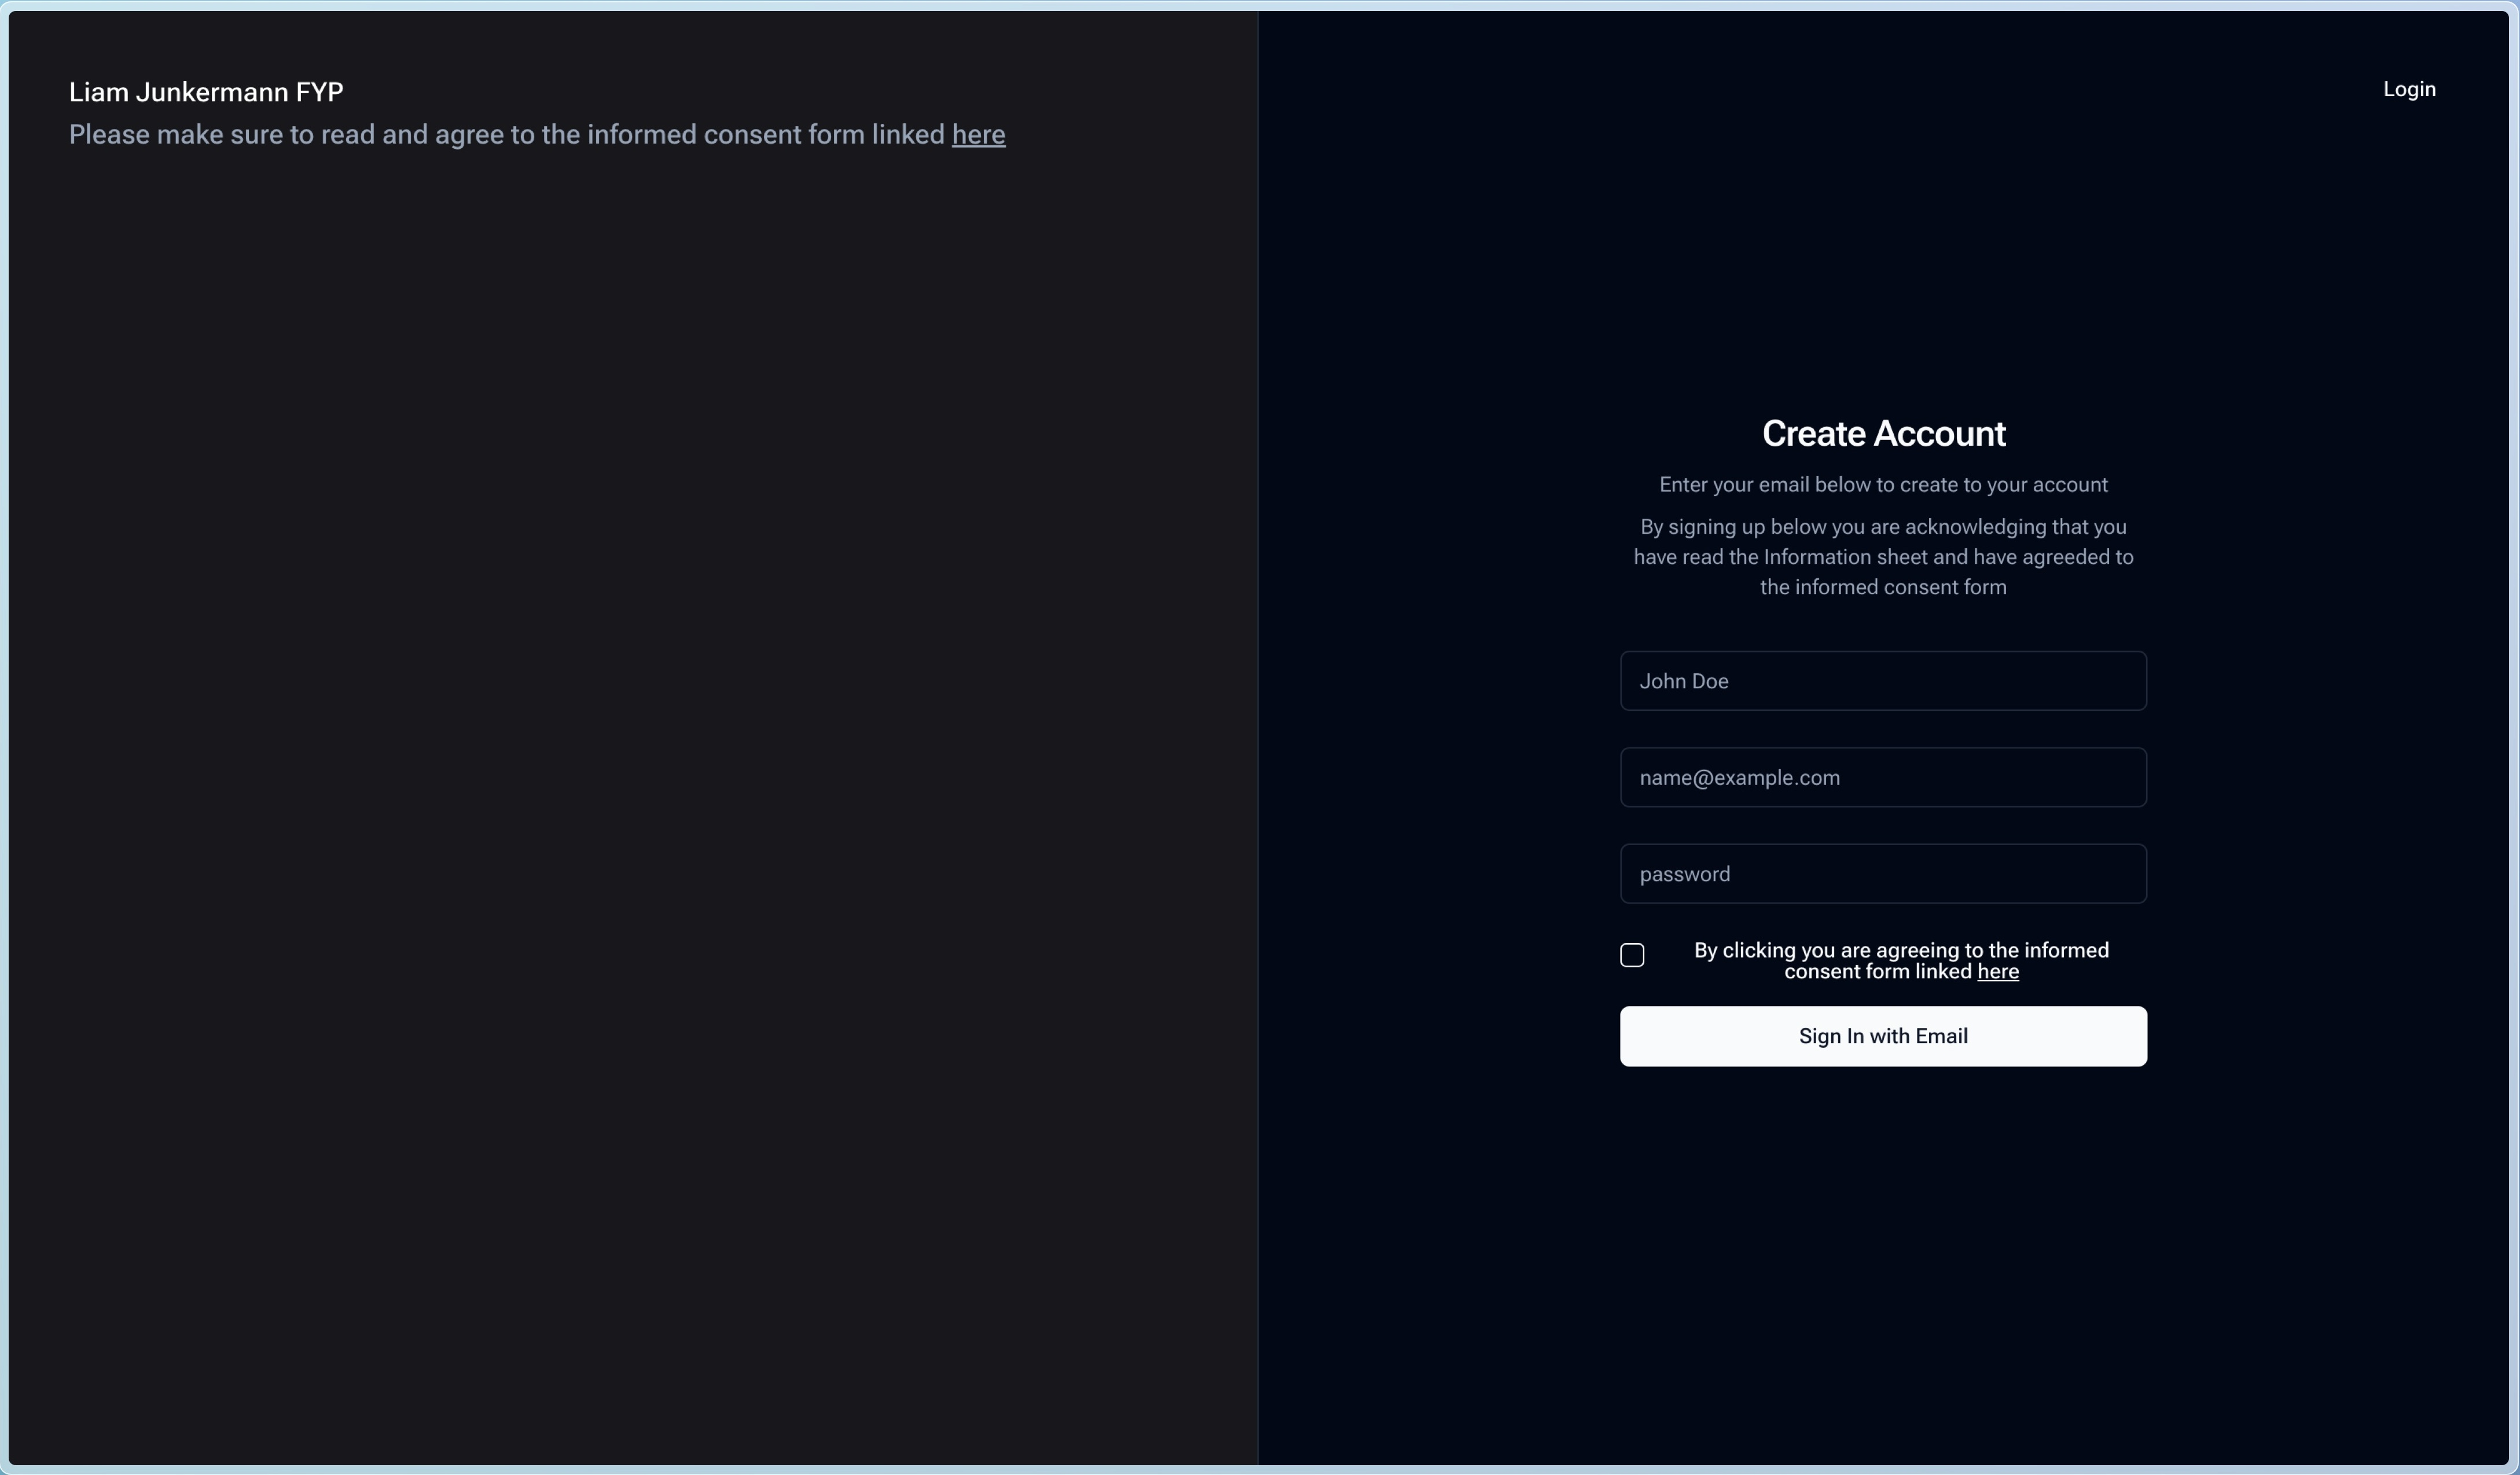
\includegraphics[width=\textwidth]{figures/fyp_register.jpeg}
  \captionsetup{justification=centering}
  \caption*{The user registration screen for the web app} \label{fig:app_webapp_register}
\end{figure}
\begin{figure}[!hp]
  \centering
  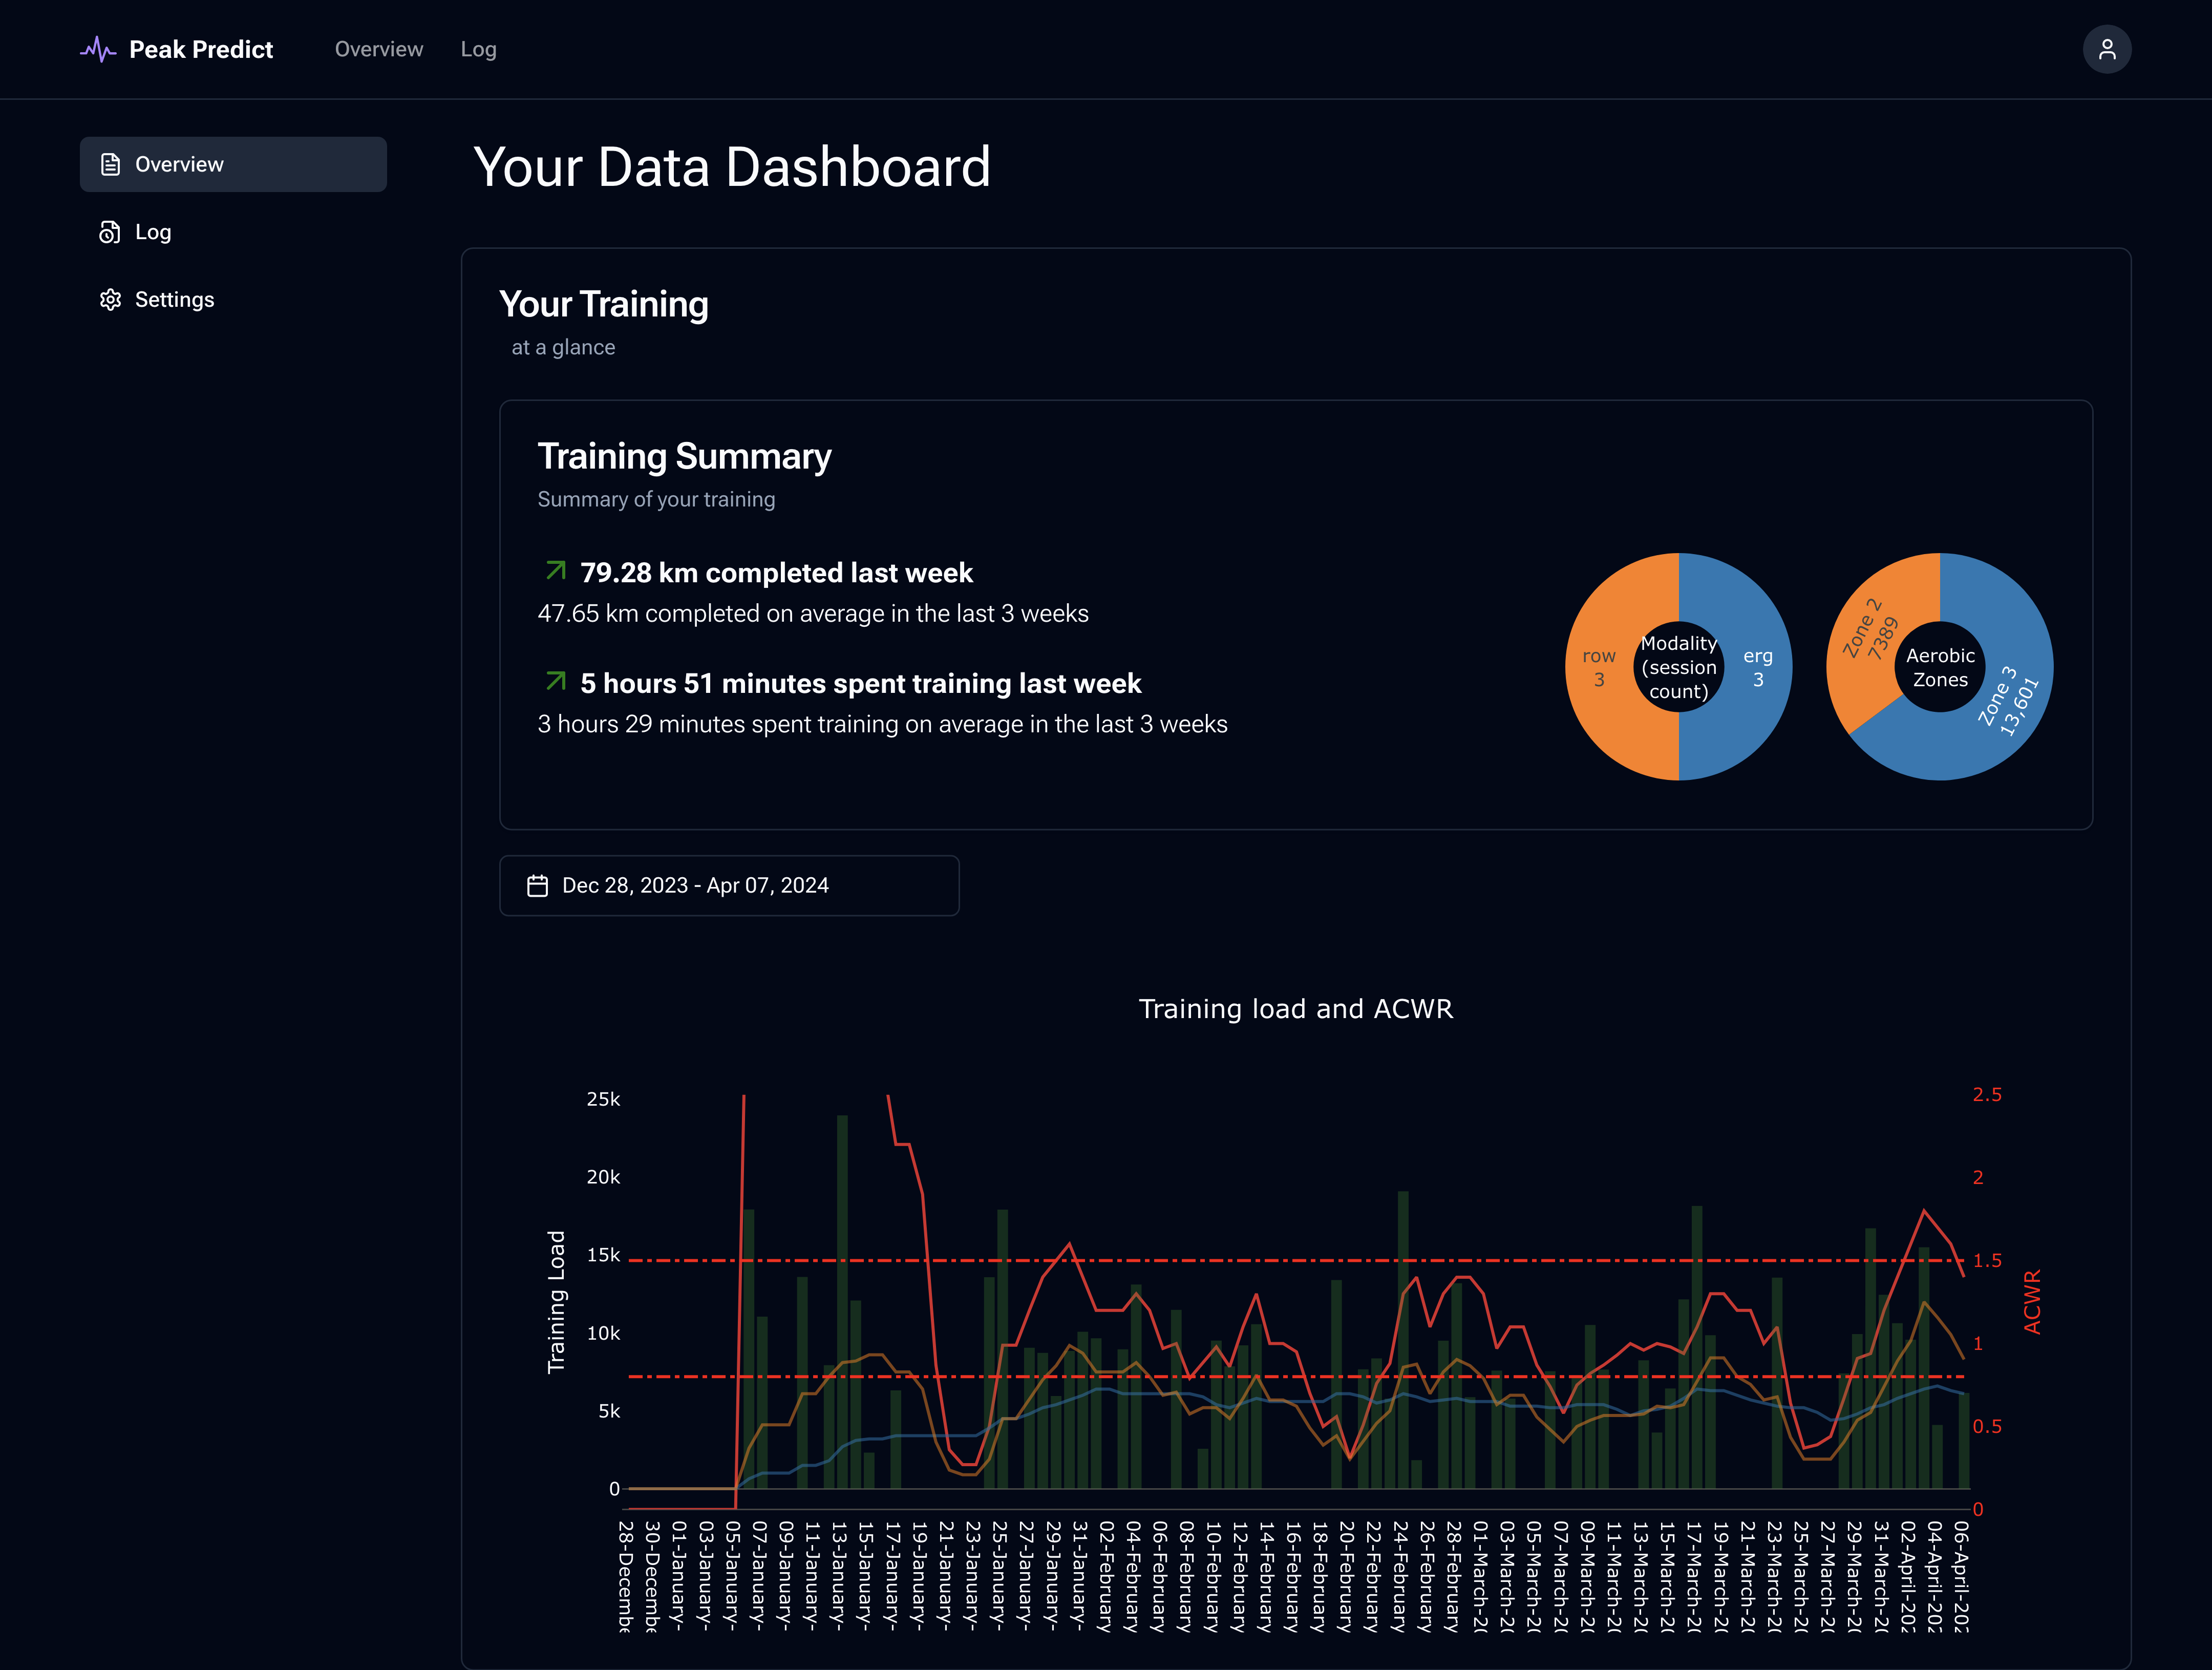
\includegraphics[width=\textwidth]{figures/fyp_dash_overview.png}
  \captionsetup{justification=centering}
  \caption*{The dashboard screen for the web app} \label{fig:app_webapp_dashboard}
\end{figure}
\begin{figure}[!hp]
  \centering
  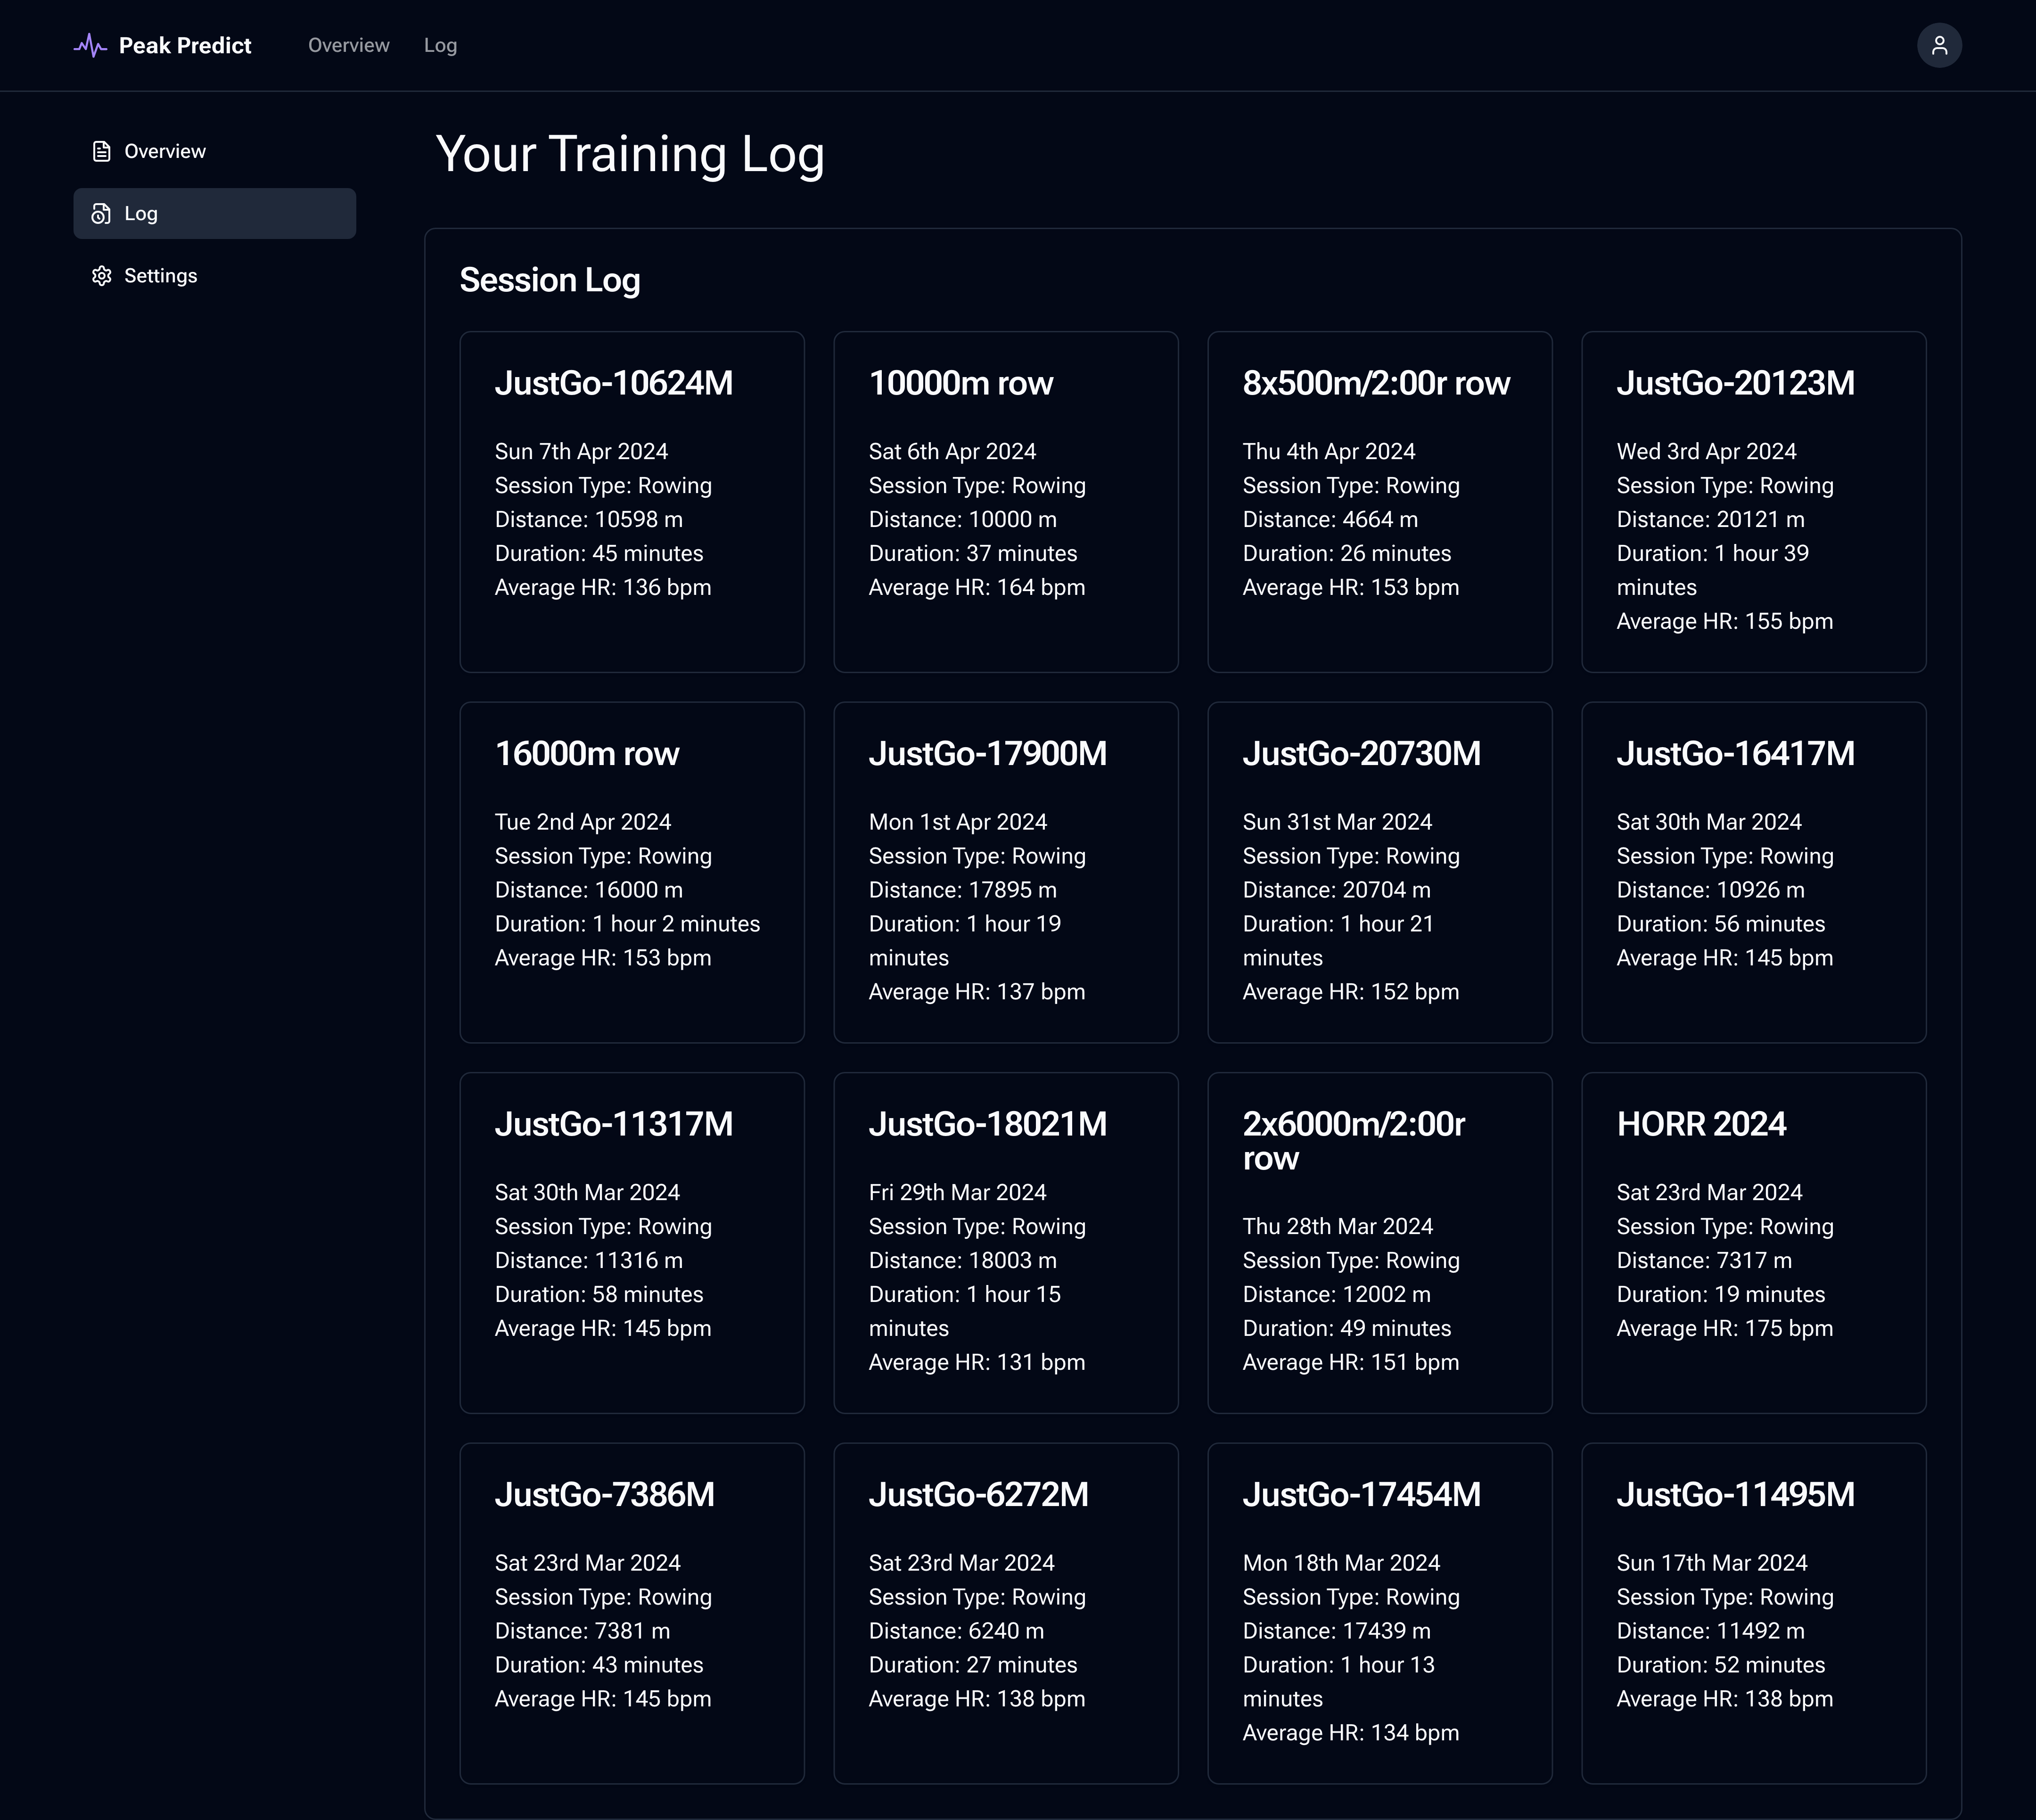
\includegraphics[width=\textwidth]{figures/fyp_training_log.png}
  \captionsetup{justification=centering}
  \caption*{The training log screen for the web app with 16 sessions loaded} \label{fig:app_webapp_training_log}
\end{figure}
\begin{figure}[!hp]
  \centering
  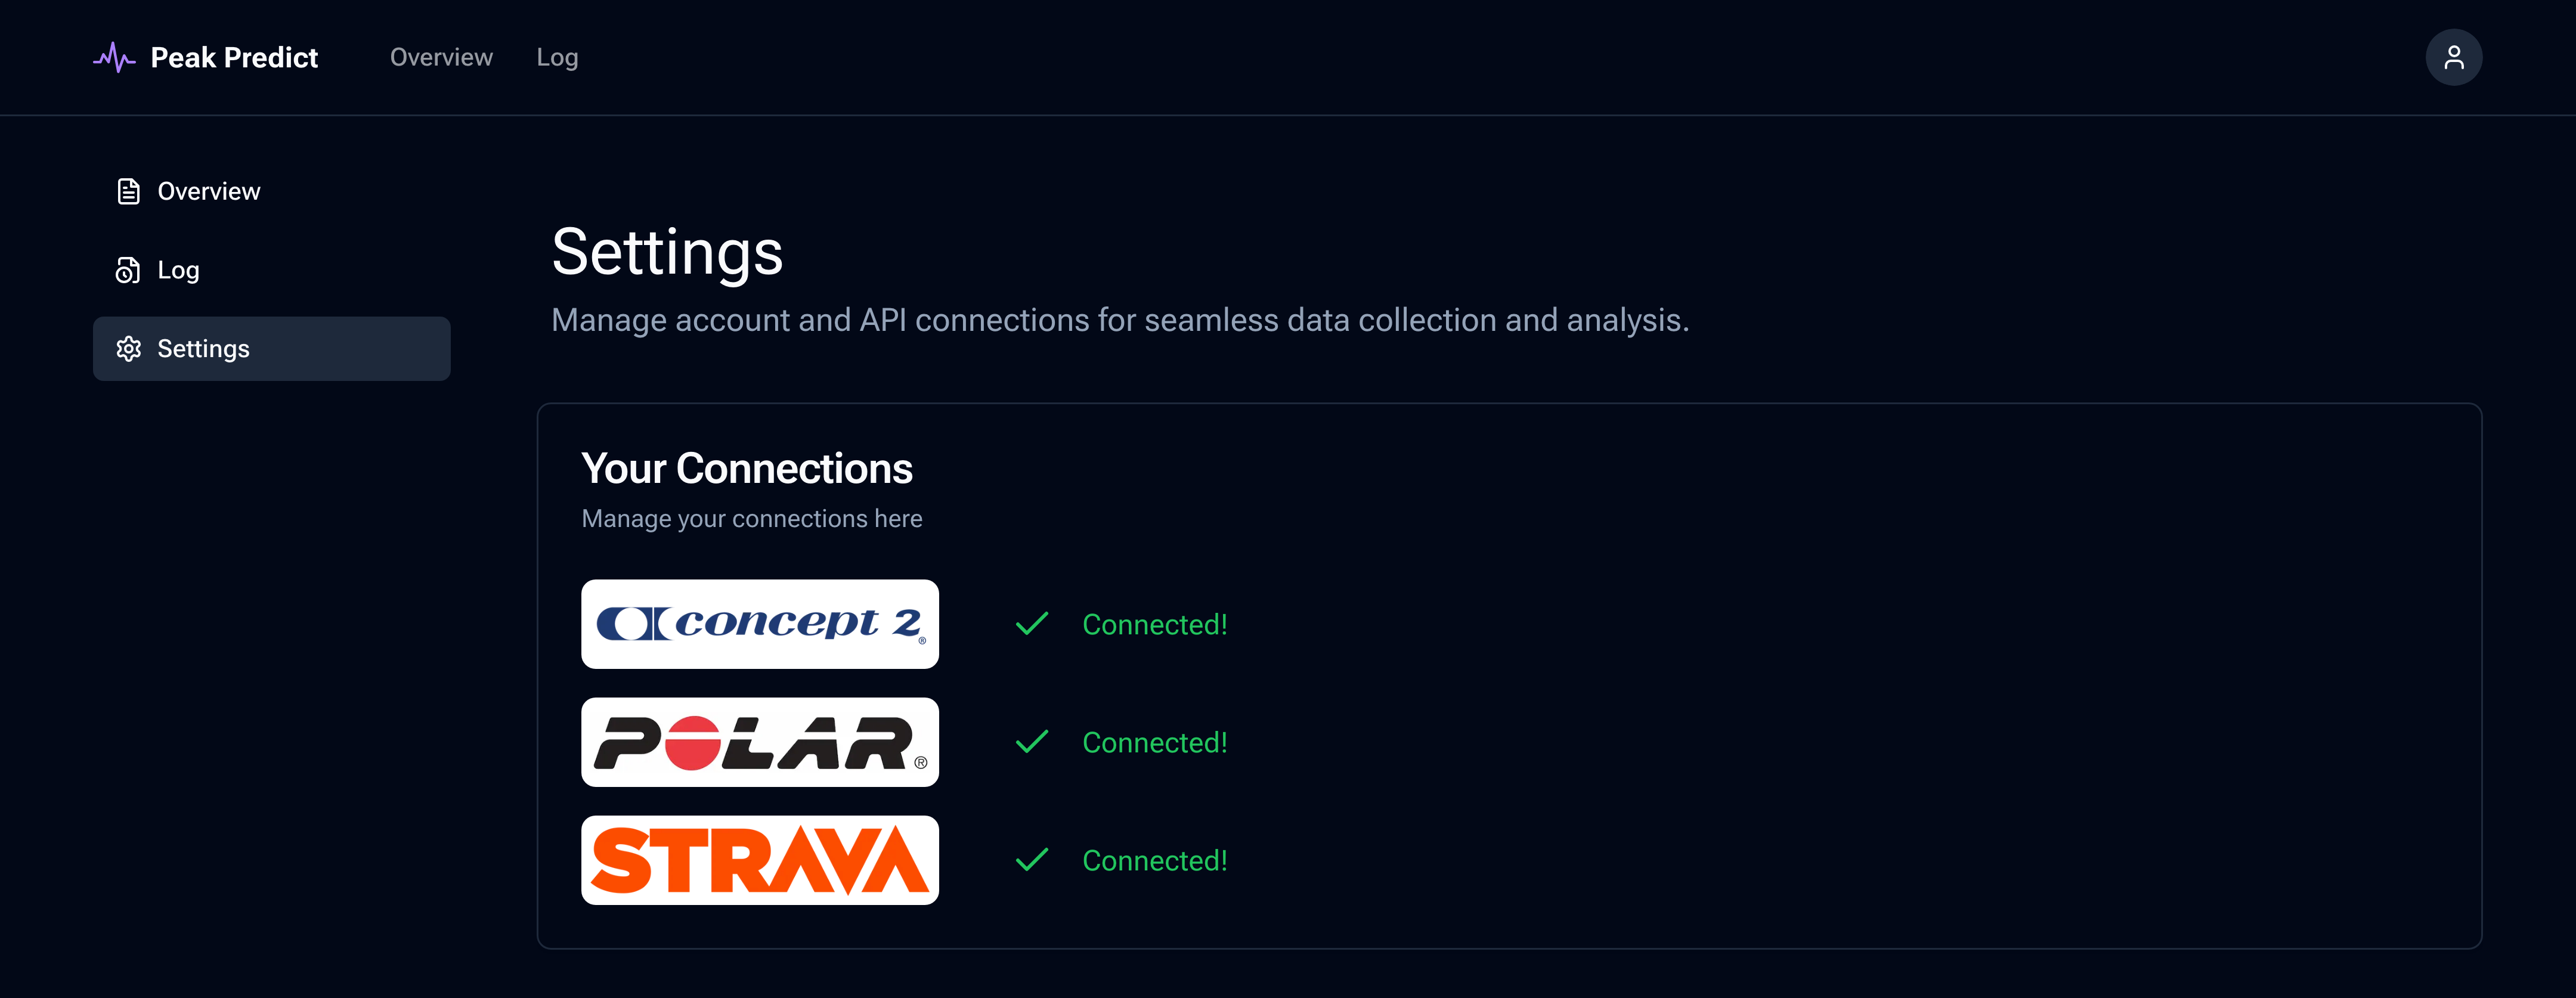
\includegraphics[width=\textwidth]{figures/fyp_connections_page.png}
  \captionsetup{justification=centering}
  \caption*{\label{fig:app_webapp_connection_mgr}The connections manager screen for the web app} 
\end{figure}

\newpage
\section{Visualisations}
\begin{figure}[!hp]
  \centering
  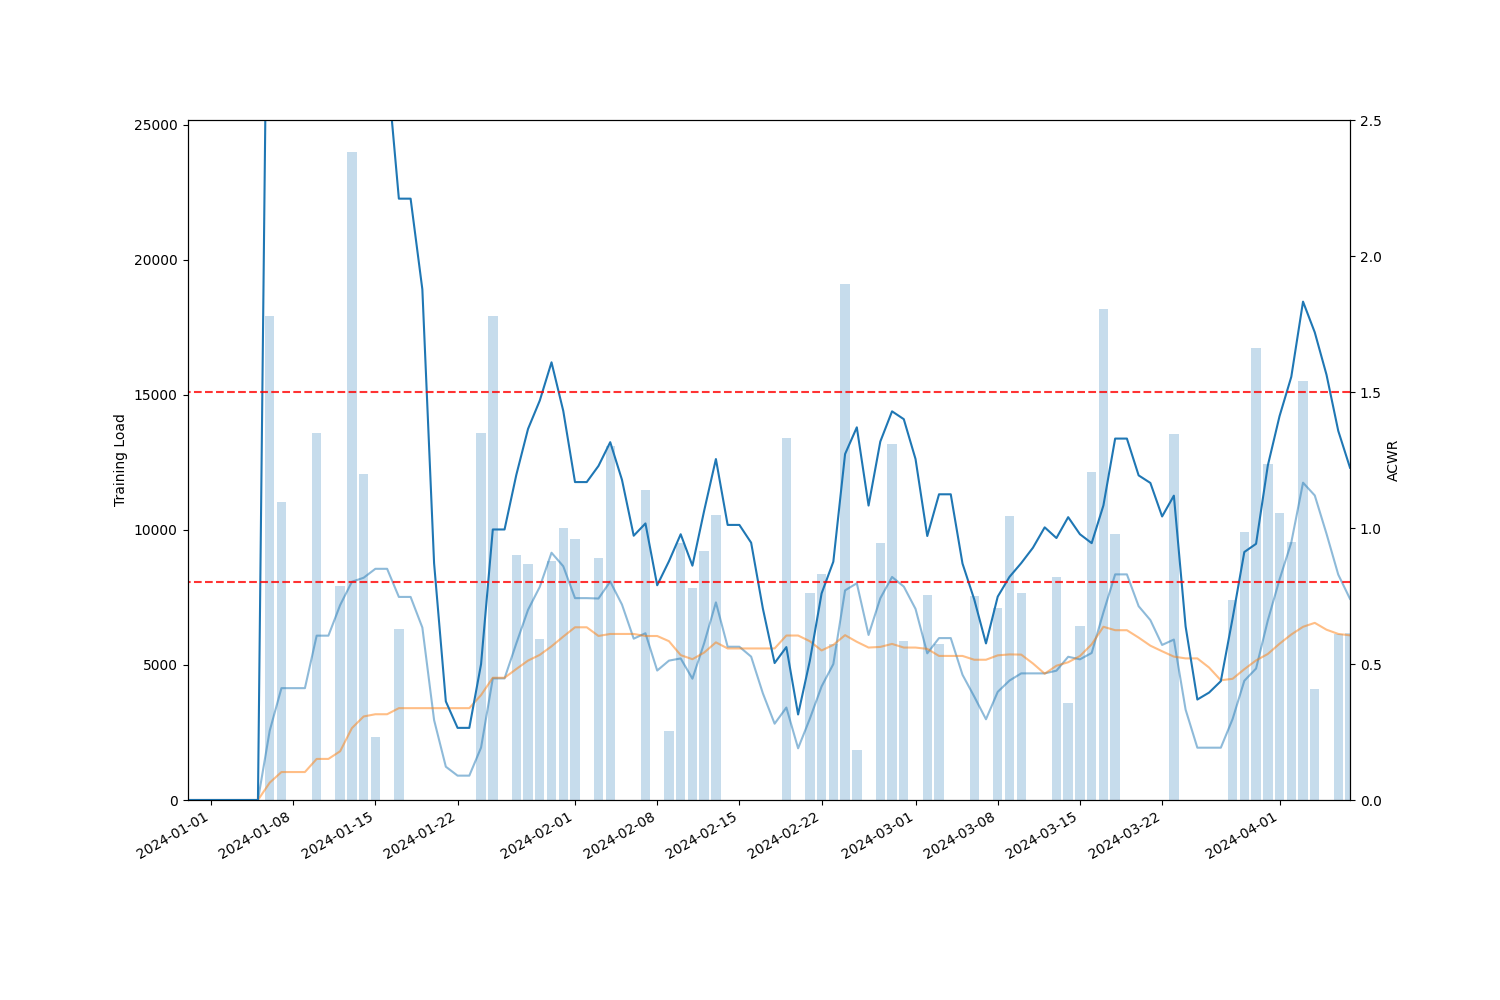
\includegraphics[width=\linewidth]{figures/acwr.png}
  \captionsetup{justification=centering}
  \caption*{\label{fig:app_acwr}The Acute, Chronic, TRIMP, ACWR chart}
\end{figure}
\begin{figure}[!hp]
  \centering
  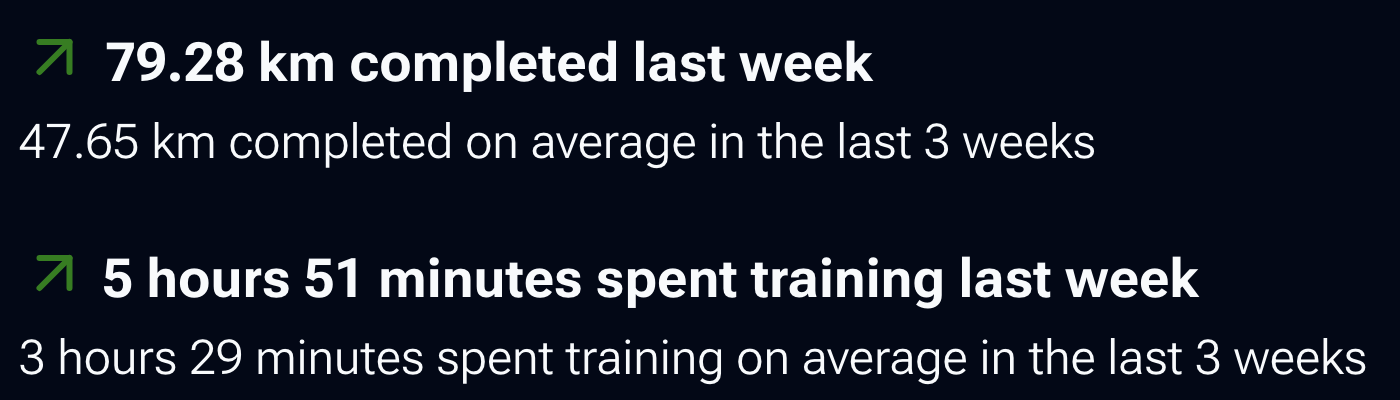
\includegraphics[width=\linewidth]{figures/trainingOverviewWidget.png}
  \captionsetup{justification=centering}
  \caption*{\label{fig:app_weeklyTrainingOverview}The weekly training overview widget, comparing the last weeks mileage and training time to the average of the previous 3 weeks} 
\end{figure}
\begin{figure}[!hp]
  \centering
  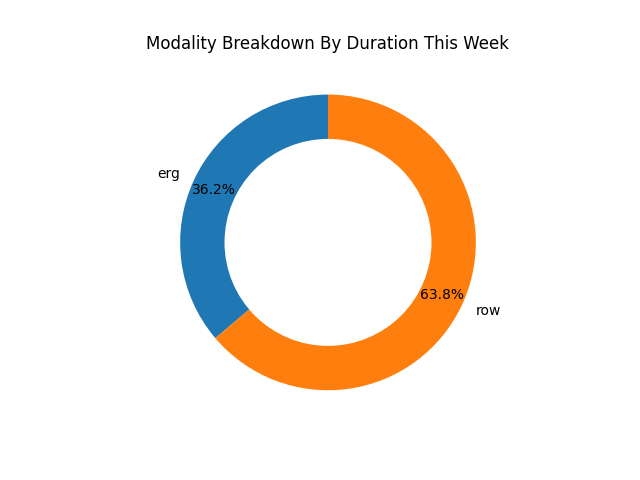
\includegraphics[width=\linewidth]{figures/durationDonut.png}
  \captionsetup{justification=centering}
  \caption*{\label{fig:app_durationDonut}A donut graph showing the distribution of training duration across different modalities}
\end{figure}
\begin{figure}[!hp]
  \centering
  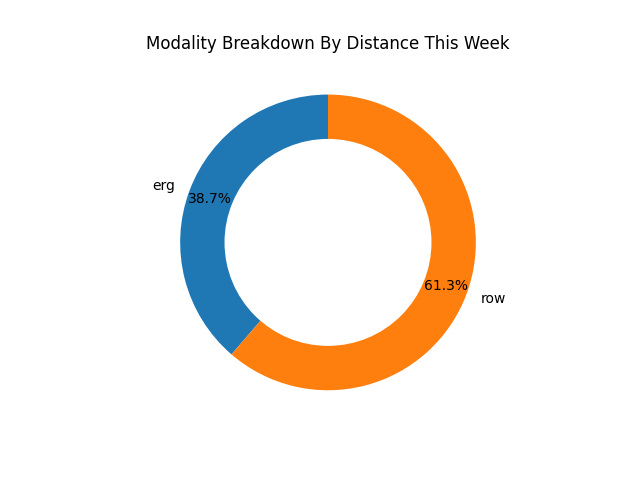
\includegraphics[width=\linewidth]{figures/distanceDonut.png}
  \captionsetup{justification=centering}
  \caption*{\label{fig:app_distanceDonut}A donut graph showing the distribution of training distance across different modalities}
\end{figure}
\begin{figure}[!hp]
  \centering
  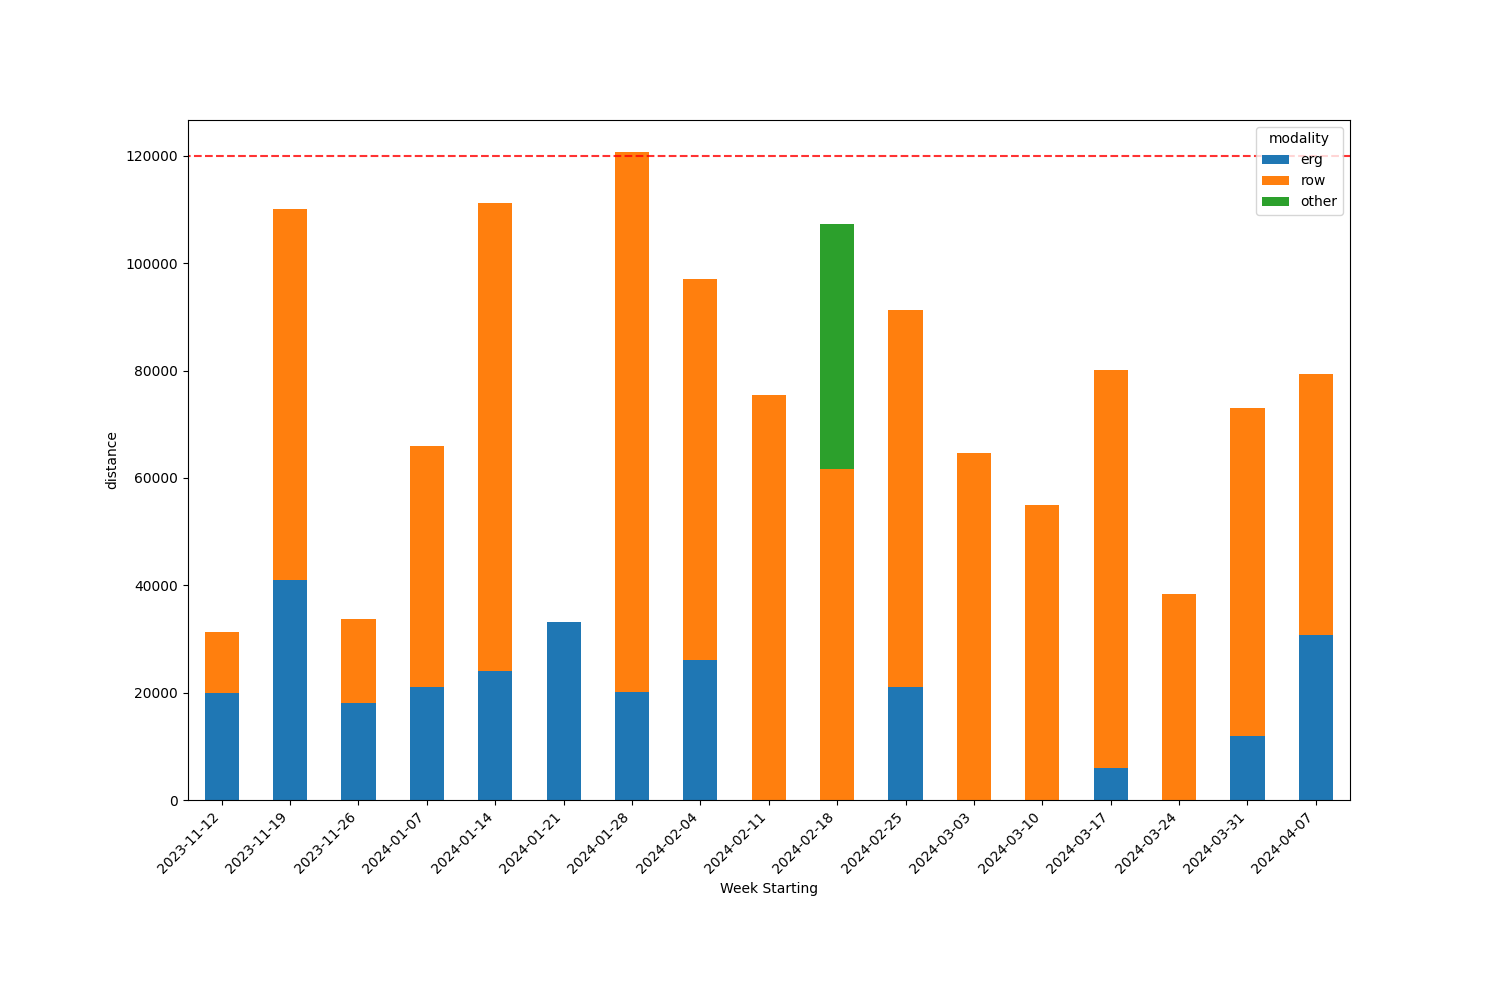
\includegraphics[width=\linewidth]{figures/distanceVsMod.png}
  \captionsetup{justification=centering}
  \caption*{\label{fig:app_distanceVsMod}A stacked bar chart showing the weekly distance completed across different modalities}
\end{figure}
\begin{figure}[!hp]
  \centering
  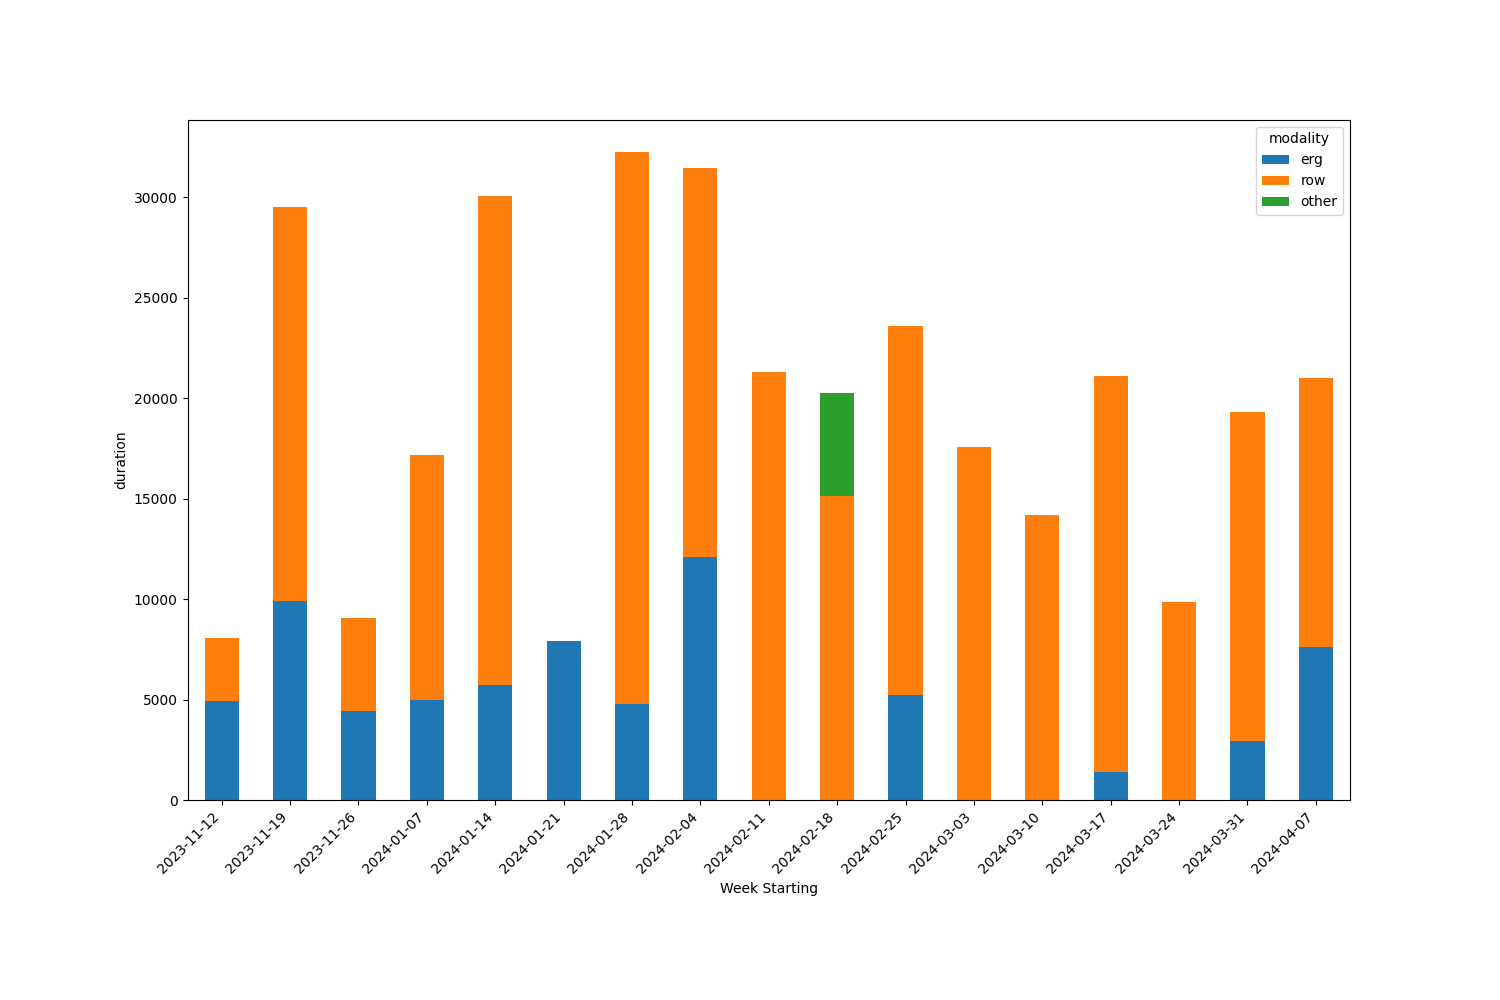
\includegraphics[width=\linewidth]{figures/durationVsMod.png}
  \captionsetup{justification=centering}
  \caption*{\label{fig:app_durationVsMod}A stacked bar chart showing the weekly duration completed across different modalities}
\end{figure}


\newpage
\section{\label{sec:ethics-approval-application}Ethics Approval Application}
The Ethics Approval Application, which was submitted on November 2, 2023, and approval was granted on December 6, 2023, is attached on the following 9 pages.
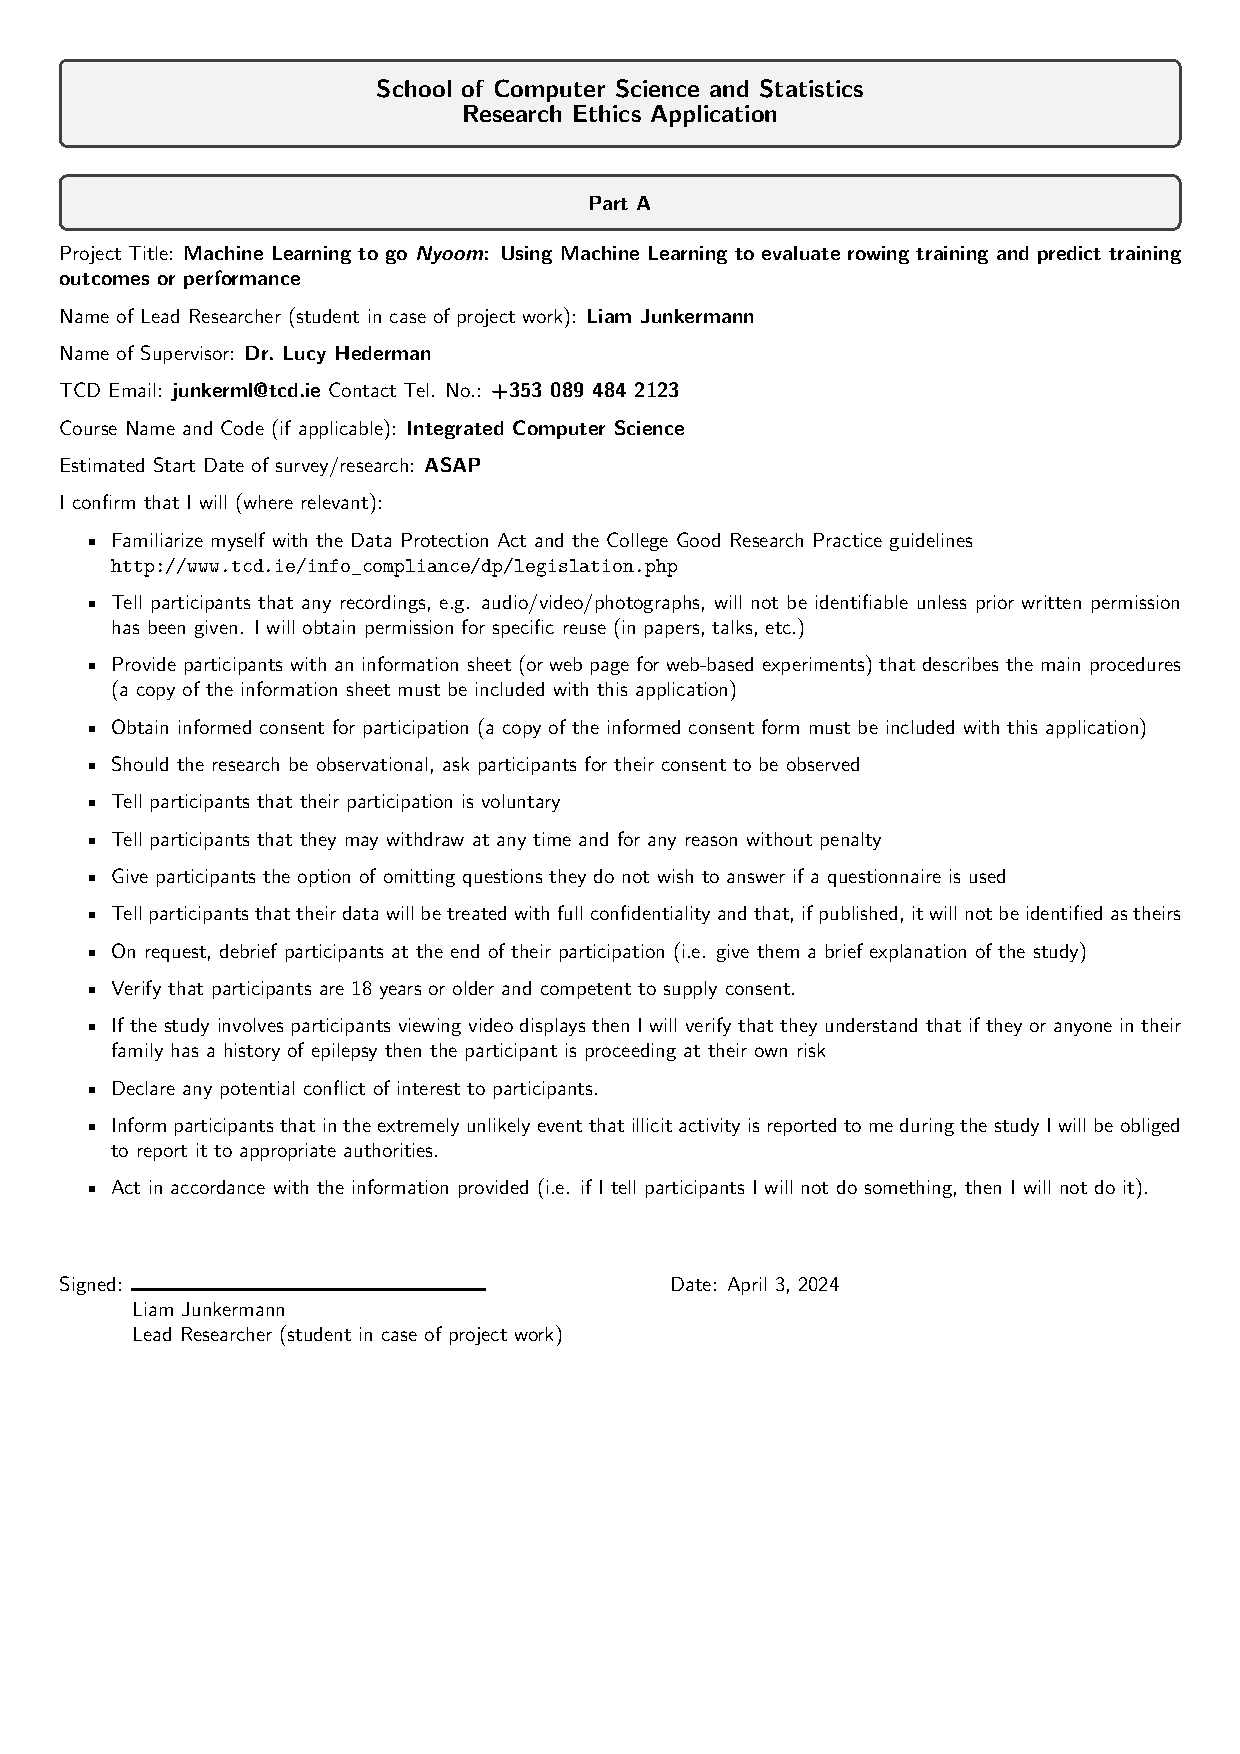
\includepdf[pages=-]{appendix/LiamJunkermannEthicsProposal.pdf}